\documentclass[14pt]{article}

\usepackage[utf8x]{inputenc}
\usepackage[russian]{babel}
\usepackage{graphicx}
\graphicspath{{images/}}
\DeclareGraphicsExtensions{.pdf,.png,.jpg}

\usepackage{amsmath}
\usepackage{pgfplots}

\usepackage{geometry} % Меняем поля страницы
\geometry{left=2cm}% левое поле
\geometry{right=1.5cm}% правое поле
\geometry{top=2cm}% верхнее поле
\geometry{bottom=2cm}% нижнее поле

\renewcommand{\theenumi}{\arabic{enumi}}
\renewcommand{\labelenumi}{\arabic{enumi}}
\renewcommand{\theenumii}{.\arabic{enumii}}
\renewcommand{\labelenumii}{\arabic{enumi}.\arabic{enumii}.}
\renewcommand{\theenumiii}{.\arabic{enumiii}}
\renewcommand{\labelenumiii}{\arabic{enumi}.\arabic{enumii}.\arabic{enumiii}.}

\begin{document}
\begin{titlepage}
	\begin{center}
		\fontsize{18pt}{20pt}\selectfont
		\textbf{Работа 3.6.1.}	
	
		\vspace{5cm}
		\fontsize{24pt}{25pt}\selectfont
		Спектральный анализ электрических сигналов. 
	\end{center}
	\begin{flushright}
		\fontsize{18pt}{20pt}\selectfont
		\vspace{14cm}
		\hspace{-3cm}
		\textit{Корнеев Е.С.}
	\end{flushright}		
\end{titlepage}

\begin{center}
	\fontsize{16pt}{18pt}\selectfont	
	Спектральный анализ электрических сигналов. 
\end{center}


\fontsize{14pt}{16pt}\selectfont
\vspace{1cm}
\textbf{Цель работы:} изучение спектрального состава периодических электрических сигналов.

\vspace{0.5cm}
\textbf{Оборудование:} персональный компьютер, USB-осциллограф АКИП-4107, функциональный генератор WaveStation 2012, соединительные кабели.

\vspace{1cm}

Многие физические процессы можно моделировать с помощью линейных дифференциальных уравнений. К решениям таких уравнений применим принцип суперпозиции: разнообразные сложные явления удобно представлять в виде суммы простых решений линейных уравнений. Для линейных уравнений такими простыми решениями являются гармонические функции. Математическая теория представления сложных функций в виде сумм гармонических составляющих получила название теории рядов и интегралов Фуръе.

В радиотехнике широко используется разложение сложных сигналов на гармонические колебания различных частот $\omega$. Функция $F(\omega)$‚ описывающая зависимость амплитуды гармоник от их частоты, называется \textsl{амплитудной спектральной характеристикой} - спектром исходного сигнала. Представление сложного периодического сигнала в виде суммы гармонических сигналов в математике называется разложением в ряд Фуръе. Непериодические сигналы представляются в виде интеграла Фурье.

Пусть заданная функция $f(t)$ периодически повторяется с частотой $\Omega_1 = 2\pi/T$, где $T$ - период повторения. Ее разложение в ряд Фурье имеет вид
\begin{equation}
f(t) = \frac{a_0}{2} + \sum_{i = 1}^{\infty}[a_n\cos(n\Omega_1t) + b_n\sin(n\Omega_2t)]
\end{equation}
или
\begin{equation}
f(t) = \frac{A_0}{2} + \sum_{i = 1}^{\infty}A_n\cos(n\Omega_1t - \psi_n).
\end{equation}
\noindent где $a_0/2 = A_0/2$ - среднее значение $f(t)$, $a_n$ и $b_n$ - амплитуды членов разложения, определяющиеся по формулам
$$
	a_n = \frac{2}{T}\int_{t_1}^{t_1 + T}f(t)\cos(n\Omega_1t)dt,
$$
$$
	b_n = \frac{2}{T}\int_{t_1}^{t_1 + T}f(t)\sin(n\Omega_1t)dt,
$$
\noindent точку $t_1$ можно выбрать произвольно. При этом между коэффициентами существует следующая связь:
$$
	A_n = \sqrt{a_n^2 + b_n^2};~~~\psi_n = \arctan\frac{b_n}{a_n}
$$
\noindent Таким образом, видно, что сигнал раскладывается в сумму сигналов с частотами $\Omega_1$, $2\Omega_1$, $3\Omega_1$, и т.д. Представляя $\cos\alpha$ в виде
$$
	\cos\alpha = \frac{e^{i\alpha} + e^{-i\alpha}}{2}
$$
\noindent и подставляя в (2):
$$
	f(t) = \frac{1}{2}\left(A_0 + \sum_{n = 1}^{\infty}A_ne^{-i\psi_n}e^{in\Omega_1t} + \sum_{n = 1}^{\infty}A_ne^{i\psi_n}e^{-in\Omega_1t}\right)
$$
\noindent Вводя комплексные амплитуды
\begin{equation}
\widetilde{A_n} = A_ne^{-i\psi_n};~~\widetilde{A_{-n}} = A_ne^{i\psi_n};~~\widetilde{A_0} = A_0
\end{equation}
\noindent получим
\begin{equation}
f(t) = \frac{1}{2}\sum_{n = -\infty}^{\infty}\widetilde{A_n}e^{in\Omega_1t}
\end{equation}

 
Видно, что введение отрицательных частот ($-n\Omega_1$) позволяет записать разложение Фурье простым способом. (3) обеспечивают действительность суммы (4): каждой частоте 
$k\Omega_1$ соответствует в (2) один член ($n = k$), а в (4) - два ($n = k$ и $n = -k$). Формулы (3) позволяют переходить от комплексного представления и обратно. 

Для рассчета комплексных амплитуд умножим левую и правую части (4) на $e^{-ik\Omega_1t}$ и проинтегрируем за период, например, от 0 до $2\pi/\Omega_1$. В правой части обнулятся все члены, кроме $n = k$, дающего $A_kT/2$. Поэтому
$$
	A_k = \frac{2}{T}\int_0^Tf(t)e^{-ik\Omega_1t}dt.
$$

Теперь рассмотрим функции, исследуемые в работе.

\vspace{1cm}
\textbf{Периодическая последовательность прямоугольных сигналов} с амплитудой $V_0$, длительностью $\tau$, частотой повторения $f_{\text{повт}} = 1/T$, где $T$ - период повторения импульсов. 

\begin{figure}[h!]
	\center{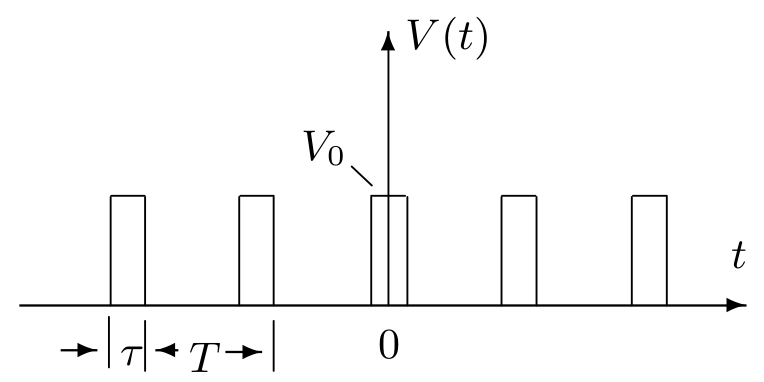
\includegraphics[width = 10cm]{1}}
	\caption{Периодическая последовательность прямоугольных импульсов}
	\label{fig:image}
\end{figure}

Найдем среднее значение:
$$
	\langle V\rangle = \frac{a_0}{2} = \frac{A_0}{2} = \frac{1}{T}\int_{-\tau/2}^{\tau/2}V_0dt = V_0\frac{\tau}{T}
$$

Амплитуды косинусных составляющих будут равны
$$
	a_n = \frac{2}{T}\int_{-\tau/2}^{\tau/2}V_0\cos(n\Omega_1t)dt = 2V_0\frac{\tau}{T}\frac{\sin(n\Omega_1\tau/2)}{n\Omega_1\tau/2} \sim \frac{\sin(x)}{x}
$$

\begin{figure}[h!]
	\center{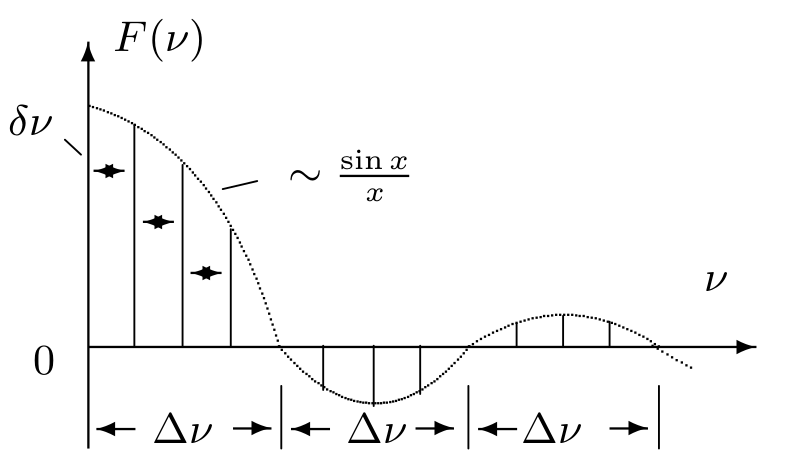
\includegraphics[width = 10cm]{2}}
	\caption{Спектр периодической последовательности прямоугольных импульсов}
	\label{fig:image}
\end{figure}

Поскольку функция четная, все амплитуды синусоидальных гармоник будут нулевыми. Амплитуды гармоник меняются по закону $\frac{\sin(x)}{x}$. На графике изображен случай, когда $T$ крастно $\tau$. Назовем шириной спектра $\Delta\nu$ расстояние от первого максимума, возникающего от главного максимума до первого нуля, возникающего при 
$\Omega_1 = 2\pi/T$. При этом $\Delta\omega\tau \approx 2\pi$, или $\Delta\nu\Delta t \approx 1$.

\vspace{1cm}
\textbf{Периодическая последовательность цугов} гармонического колебания $V_0\cos(\omega_0t)$ с длительностью цуга $\tau$ и периодом повторения $T$. 

\begin{figure}[h!]
	\center{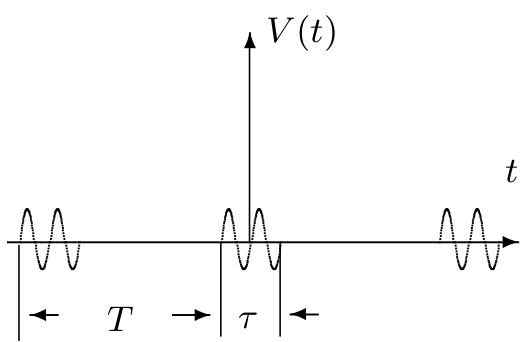
\includegraphics[width = 10cm]{3}}
	\caption{Периодическая последовательность цугов}
	\label{fig:image}
\end{figure}

Функция также симметричная относительно $t = 0$. Амплитуда $n-$й гармоники определяется выражением
$$
	A_n = a_n = \frac{2}{T}\int_{-\tau/2}^{\tau/2}V_0\cos(\omega_0t)\cdot\cos(n\Omega_1t)dt = 
$$
$$
	= V_0\frac{\tau}{T}\left(\frac{\sin[(\omega_0 - n\Omega_1)\frac{\tau}{2}]}{(\omega_0 - n\Omega_1)\frac{\tau}{2}} + 
	                         \frac{\sin[(\omega_0 + n\Omega_1)\frac{\tau}{2}]}{(\omega_0 + n\Omega_1)\frac{\tau}{2}}
	                   \right)
$$

\begin{figure}[h!]
	\center{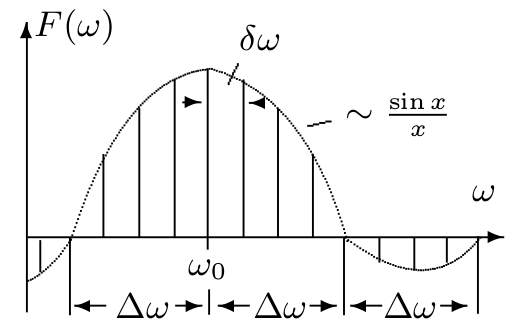
\includegraphics[width = 10cm]{4}}
	\caption{Спектр периодической последовательности цугов}
	\label{fig:image}
\end{figure}

Такое спектральное распределение $F(\omega)$ для случая, когда $T$ кратно $\tau$, представлено на рис. 5. Сравнивая этот график с аналогичным для прямоугольных импульсов, видим, что они аналогичны, но максимумы сдвинуты на почастоте на $\omega_0$. 

\vspace{1cm}
\textbf{Амплитудно-модулированные сигналы}. Рассмотрим гармонические колебания частоты $\omega_0$, амплитуда которых медленно меняется по гармоническому закону с частотой 
$\Omega$ ($\Omega \ll \omega_0$):
\begin{equation}
f(t) = A_0[1 + m\cos(\Omega t)]\cos(\omega t)
\end{equation}

\begin{figure}[h!]
	\center{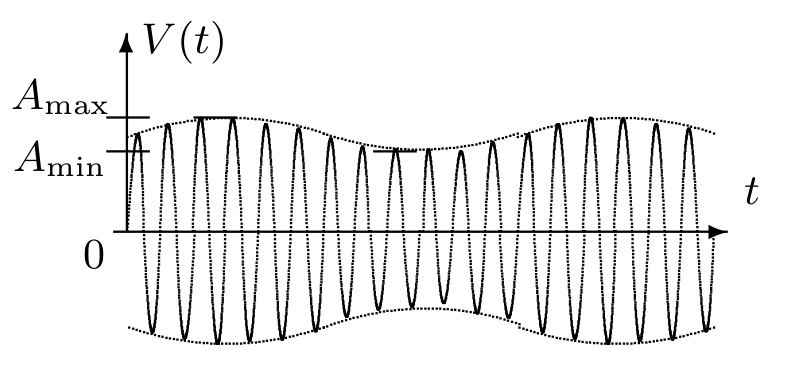
\includegraphics[width = 10cm]{5}}
	\caption{Гармонические колебания, модулированные по амплитуде}
	\label{fig:image}
\end{figure}

Коэффициент $m$ называется глубиной модуляции. При $m < 1$ амплитуда колебаний меняется от минимальной $A_{min} = A_0(1 - m)$ до максимальной $A_{max} = A_0(1 + m)$. Глубина модуляции может быть представлена в виде 
$$
	m = \frac{A_{max} - A_{min}}{A_{max} + A_{min}}
$$

Преобразовывая уравнение (5), получим спектр:
$$
	f(t) = A_0\cos(\omega_0t) + A_0m\cos(\Omega t)\cos(\omega_0t) = 
$$
$$
	= A_0\cos(\omega_0t) + \frac{A_0m}{2}\cos(\omega + \Omega)t + \frac{A_0m}{2}\cos(\omega - \Omega)t
$$

\begin{figure}[h!]
	\center{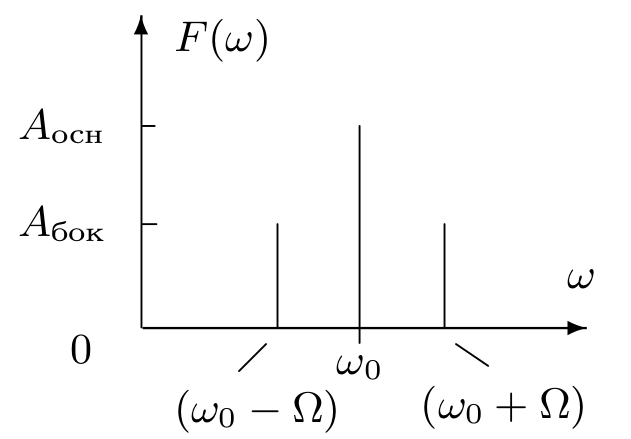
\includegraphics[width = 10cm]{6}}
	\caption{Спектр гармонических колебания, модулированных по амплитуде}
	\label{fig:image}
\end{figure}

Спектр $F(\omega)$ таких колебаний содержит три составляющих. Основная компонента представляет собой исходное немодулированное колебание с несущей частотой $\omega_0$ и амплитудой $A_{\text{осн}} = A_0$ - первое слагаемое в правой части последнего уравнения. Боковые компоненты спектра соответствуют гармоническим колебаниям с частотами 
($\omega_0 + \Omega$) и ($\omega_0 - \Omega$) - второе и третье слагаемые. Амлитуды этих колебаний одинаковы и составляют $m/2$ от амплитуды немодулированного сигнала:
$A_{\text{бок}} = A_0m/2$.

\newpage
\textbf{Экспериментальная установка.} 

Функциональный генератор WaveStation 2012 позволяет сформировать два различных электрических сигнала, которые выводятся на два независимых канала – CH1 и CH2. Сигнал с канала CH1 подается на вход А, а сигнал с канала CH2 – на вход В USB-осциллографа. Затем эти сигналы подаются на вход компьютера через USB-соединение. При работе USB- осциллографа в режиме осциллографа, на экране компьютера можно наблюдать каждый из сигналов в отдельности, а также их произведение. В режиме спектроанализатора можно наблюдать спектры этих сигналов. При включении функционального генератора, на его экране отображается информация о параметрах электрического сигнала.

\begin{figure}[h!]
	\center{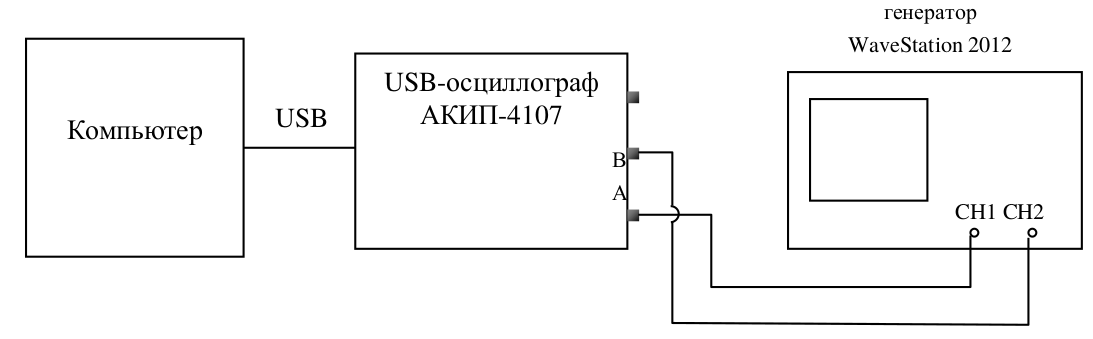
\includegraphics[width = 16cm]{fac_main}}
	\caption{Схема для исследования сигналов}
	\label{fig:image}
\end{figure}

\newpage
\textbf{А. Исследование спектра периодической последовательности прямоугольных импульсов}
\vspace{1cm}
\textbf{Ход работы:}

1. Получим на экране спектр импульсов с параметрами $f_{\text{повт}} = 10^3$ Гц; $\tau = 25$ мкс. Первый ноль амплитуды наблюдается ни $\nu = 10$ кГц. При увеличении $\tau$ вдвое мы наблюдаем уменьшение нуля амплитуды до $5$ кГц, при увеличении $f_{\text{повт}}$ вдвое ноль не меняется, зато возрастает аплитуда сигнала.

2. Снимем зависимость ширины спектра $\Delta\nu$ от длительности импульса $\tau$:

\begin{center}
\begin{tabular}{|c|c|c|c|c|}
\hline
$\tau$, мкс&$\Delta\nu$, кГц&$1/\tau$, мкс$^{-1}$\\
\hline
40.0&26.0&0,025\\
\hline
60.0&17.0&0,017\\
\hline
80.0&12.0&0,013\\
\hline
100.0&10.0&0,010\\
\hline
120.0&8.0&0,008\\
\hline
140.0&7.0&0,007\\
\hline
160.0&6.0&0,006\\
\hline
180.0&6.0&0,006\\
\hline
200.0&5.0&0,005\\
\hline
\end{tabular}
\end{center}

В данном случае примем погрешность $\sigma_\tau$ равной 0.1 мкс, так как мы имеем возможность выставлять $\tau$ на генераторе с точностью до десятых. Соответственно, погрешность $1/\tau$ будет пренебрежимо мала, т.к., вычисленная по формуле
$$
	\sigma_{1/\tau} = \frac{1}{\tau}\cdot \varepsilon_\tau,
$$
\noindent она составляет доли процентов от величины, и в данном случае может не учитываться, так как она на два порядка меньше, чем порядок значащих цифр. Погрешность $\sigma_\nu$ примем равной 0.5 кГц, так как деления на шкале спектрометра на экране не позволяют измерять с большей точностью.

Таким образом, можем построить график $\Delta\nu(1/\tau)$:

\vspace{1cm}
\begin{tikzpicture}
\begin{axis}[
	height = 10cm,
	width  = 15cm,
	every axis y label/.style={at = {(ticklabel cs: 0.5)}, rotate = 90, anchor = near ticklabel},
	xlabel = {$1/\tau,$ мкс$^{-1}$},
	ylabel = {$\Delta\nu$, кГц},
	grid   = major,
]
\addplot+[
	only marks,
	error bars/.cd, 
	y dir = both, y explicit,
	x dir = both, x explicit,
	]
coordinates{
	(0.025, 26)		+-	(0, 0.5)
	(0.017, 17)		+-	(0, 0.5)
	(0.013, 12)		+-	(0, 0.5)
	(0.010, 10)		+-	(0, 0.5)
	(0.008, 8 )		+-	(0, 0.5)
	(0.007, 7 )		+-	(0, 0.5)
	(0.006, 6 )		+-	(0, 0.5)
	(0.006, 6 )		+-	(0, 0.5)
	(0.005, 5 )		+-	(0, 0.5)
};

\addplot [mark = none, color = blue]
coordinates{
	(0.025, 25.491)
	(0.005, 4.80051)
};

\end{axis}
\end{tikzpicture}

Из графика определим угол наклона: $\frac{\Delta(\Delta\nu)}{\Delta(1/\tau)} = 1,0$. Полученное значение совпадает с теоретическим, ожидаемым значением. 

3. Снимем зависимость частот и амплитуд от номера гармоник для двух значений $\tau$: $\tau = 50$ мкс и $\tau = 100$ мкс:

\begin{center}
\begin{tabular}{|c|c|c|c|c|c|c|c|c|c|}
\hline
\multicolumn{3}{|c|}{$\tau = 50$ мкс}&\multicolumn{3}{|c|}{$\tau = 100$ мкс}\\
\hline
$~N~$&$\nu$, кГц&$A$, мВ&$~N~$&$\nu$, кГц&$A$, мВ\\
\hline
1&1&3,23&1&1&6,35\\
\hline
2&2&3,07&2&2&5,89\\
\hline
3&3&3,01&3&3&5,35\\
\hline
4&4&2,89&4&4&4,64\\
\hline
5&5&2,73&5&5&3,87\\
\hline
6&6&2,53&6&6&3,01\\
\hline
7&7&2,34&7&7&2,13\\
\hline
8&8&2,13&8&8&1,29\\
\hline
9&9&1,95&9&9&0,61\\
\hline
10&10&1,82&10&10&0,00\\
\hline
11&11&1,69&11&11&0,52\\
\hline
12&12&1,59&12&12&0,91\\
\hline
13&13&1,33&13&13&1,21\\
\hline
14&14&1,10&14&14&1,33\\
\hline
15&15&0,91&15&15&1,32\\
\hline
16&16&0,74&16&16&1,18\\
\hline
17&17&0,49&17&17&0,93\\
\hline
18&18&0,30&18&18&0,63\\
\hline
19&19&0,16&19&19&0,31\\
\hline
&&&20&20&0,00\\
\hline
\end{tabular}
\end{center}

По значениям восстановим графики, полученные на спектрографе:

\vspace{1cm}
\begin{tikzpicture}
\begin{axis}[
	height = 8cm,
	width  = 15cm,
	every axis y label/.style={at = {(ticklabel cs: 0.5)}, rotate = 90, anchor = near ticklabel},
	xlabel = {$\nu,$ кГц},
	ylabel = {$A$, мВ},
	grid   = major,
	ymin   = 0,
	xmin   = 0
]
\addplot+[
	mark = none,
	ybar,
	bar width = 5pt,
	]
coordinates{
	(1 , 3.23)
	(2 , 3.07)
	(3 , 3.01)
	(4 , 2.89)
	(5 , 2.73)
	(6 , 2.53)
	(7 , 2.34)
	(8 , 2.13)
	(9 , 1.95)
	(10, 1.82)
	(11, 1.69)
	(12, 1.59)
	(13, 1.33)
	(14, 1.10)
	(15, 0.91)
	(16, 0.74)
	(17, 0.49)
	(18, 0.30)
	(19, 0.16)
};

\end{axis}
\end{tikzpicture}
$\tau = 50$ мкс

\vspace{1cm}
\begin{tikzpicture}
\begin{axis}[
	height = 8cm,
	width  = 15cm,
	every axis y label/.style={at = {(ticklabel cs: 0.5)}, rotate = 90, anchor = near ticklabel},
	xlabel = {$\nu,$ кГц},
	ylabel = {$A$, мВ},
	grid   = major,
	ymin   = 0,
	xmin   = 0
]
\addplot+[
	mark = none,
	ybar,
	bar width = 5pt,
	]
coordinates{
	(1 , 6.35)
	(2 , 5.89)
	(3 , 5.35)
	(4 , 4.64)
	(5 , 3.87)
	(6 , 3.01)
	(7 , 2.13)
	(8 , 1.29)
	(9 , 0.61)
	(10, 0.00)
	(11, 0.52)
	(12, 0.91)
	(13, 1.21)
	(14, 1.33)
	(15, 1.32)
	(16, 1.18)
	(17, 0.93)
	(18, 0.63)
	(19, 0.31)
	(20, 0.00)
};

\end{axis}
\end{tikzpicture}
$\tau = 100$ мкс

Здесь погрешности примем равными $\sigma_A = 0.02$ мВ, так как в этих пределах колебались значения, снимаемые с экрана. Погрешность $\sigma_\nu = 0.5$ кГц, так как сетка идет с шагом 1кГц. 

\newpage
\textbf{Б. Исследование спектра периодической последовательности цугов гармонических колебаний}
\vspace{1cm}
\textbf{Ход работы:}

1. Установим длительность импульсов равной $\tau = 100$ мкс, затем $\tau = 200$ мкс. При этом резко возрастает амплитуда сигнала, а $\Delta\nu$ уменьшается с 10 до 5 кГц.

2. Установим длительность импульса $\tau = 100$ мкс. Меняя несущую частоту $\nu_0$, увидим, что значениям 10, 25 и 40 кГц соответствуют максимумы амплитуд, достигающиеся на частотах 9, 24 и 39 кГц. При этом $\Delta\nu$ остается примерно одной и той же.

3. Установим значение несущей частоты $\nu_0 = 30$ кГц, длительность импульса $\tau = 100$ мкс. Найдем $\delta\nu$ для нескольких частот повторений $f_{\text{повт}}$:	

\begin{center}
\begin{tabular}{|c|c|c|c|c|c|c|c|c|c|c|c|c|}
\hline
$f_{\text{повт}}$, кГц	&	0.5	&	1.0	&	2.0	&	4.0	&	5.0	\\
\hline
$\delta\nu$, кГц		&	0.5	&	1.0	&	2.0	&	4.0	&	5.0	\\
\hline
\end{tabular}
\end{center}

Погрешности $\sigma_{\delta\nu}$ и $\sigma_{f_{\text{повт}}}$ примем равными 0.1 кГц и 0.1 кГц соотвестветнно.

Построим график $\delta\nu(f_{\text{повт}})$:

\begin{tikzpicture}
\begin{axis}[
	height = 8cm,
	width  = 15cm,
	every axis y label/.style={at = {(ticklabel cs: 0.5)}, rotate = 90, anchor = near ticklabel},
	xlabel = {$f_{\text{повт}}$, кГц},
	ylabel = {$\delta\nu$, кГц},
	grid   = major
]
\addplot+[
	error bars/.cd, 
	y dir = both, y explicit,
	x dir = both, x explicit,
	]
coordinates{
	(0.5, 0.5)	+-	(0.1, 0.1)
	(1.0, 1.0)	+-	(0.1, 0.1)
	(2.0, 2.0)	+-	(0.1, 0.1)
	(4.0, 4.0)	+-	(0.1, 0.1)
	(5.0, 5.0)	+-	(0.1, 0.1)
};
\end{axis}
\end{tikzpicture}

\vspace{1cm}
Установим $\tau = 100$ мкс и снимем зависимость амплитуд и частот для различных гармоник для частот $f_{\text{повт}} = 1$ кГц и $f_{\text{повт}} = 2$ кГц:

\vspace{1cm}
\begin{center}
\begin{tabular}{|c|c|c|c|c|c|c|c|c|c|}
\hline
\multicolumn{3}{|c|}{$f_{\text{повт}} = 1$ кГц}&\multicolumn{3}{|c|}{$f_{\text{повт}} = 2$ кГц}\\
\hline
$N$&$\nu$, кГц&$A$, мВ&$N$&$\nu$, кГц&$A$, мВ\\
\hline
22&22&20,1&22&22&35,1\\
\hline
23&23&26,4&23&24&72,8\\
\hline
24&24&36,4&24&26&99,1\\
\hline
25&25&42,7&25&28&123,0\\
\hline
26&26&50,2&26&30&135,5\\
\hline
27&27&55,2&27&32&125,5\\
\hline
28&28&62,7&28&34&101,6\\
\hline
29&29&64,0&29&36&60,2\\
\hline
30&30&64,0&30&38&26,4\\
\hline
31&31&65,2&&&\\
\hline
32&32&60,2&&&\\
\hline
33&33&57,7&&&\\
\hline
34&34&45,2&&&\\
\hline
35&35&38,9&&&\\
\hline
36&36&32,6&&&\\
\hline
37&37&21,3&&&\\
\hline
38&38&15,1&&&\\
\hline
\end{tabular}
\end{center}

\vspace{1cm}
Восстановим графики, полученные на спектрометре:

\vspace{1cm}
\begin{tikzpicture}
\begin{axis}[
	height = 8cm,
	width  = 15cm,
	every axis y label/.style={at = {(ticklabel cs: 0.5)}, rotate = 90, anchor = near ticklabel},
	xlabel = {$\nu,$ кГц},
	ylabel = {$A$, мВ},
	grid   = major,
	ymin   = 0
]
\addplot+[
	mark = none,
	ybar,
	bar width = 5pt,
	]
coordinates{
	(22, 20.1)
	(23, 26.4)
	(24, 36.4)
	(25, 42.7)
	(26, 50.2)
	(27, 55.2)
	(28, 62.7)
	(29, 64.0)
	(30, 64.0)
	(31, 65.2)
	(32, 60.2)
	(33, 57.7)
	(34, 45.2)
	(35, 38.9)
	(36, 32.6)
	(37, 21.3)
	(38, 15.1)
};

\end{axis}
\end{tikzpicture}
$f_{\text{повт}} = 1$кГц

\vspace{1cm}
\begin{tikzpicture}
\begin{axis}[
	height = 8cm,
	width  = 15cm,
	every axis y label/.style={at = {(ticklabel cs: 0.5)}, rotate = 90, anchor = near ticklabel},
	xlabel = {$\nu,$ кГц},
	ylabel = {$A$, мВ},
	grid   = major,
	ymin   = 0
]
\addplot+[
	mark = none,
	ybar,
	bar width = 5pt,
	]
coordinates{
	(22, 35.1 )
	(23, 72.8 )
	(24, 99.1 )
	(25, 123.0)
	(26, 135.5)
	(27, 125.5)
	(28, 101.6)
	(29, 60.2 )
	(30, 26.4 )
};

\end{axis}
\end{tikzpicture}
$f_{\text{повт}} = 2$кГц

\vspace{1cm}
Теперь сравним картины спектров:

1. Прямоугольные импульсы. При увеличении $\tau$ вдвое мы наблюдаем уменьшение вдвое $\Delta\nu$.

2. Цуги. Увеличивая вдвое $f_{\text{повт}}$, мы наблюдаем уменьшение $\Delta\nu$ также вдвое.

3. Сравнивая картины спектров цугов и импульсов при равных значениях $\tau = 100$ мкс и $f_{\text{повт}} = 1$ кГц, видим, что максимум амплитуды цугов находится заметно правее максимума импульсов.


\newpage
\textbf{В. Исследование спектра гармонических колебаний, модулированных по амплитуде}
\vspace{1cm}
\textbf{Ход работы:}

Снимем зависимость $A_{max}$, $A_{min}$, $A_{\text{осн}}$, $A_{\text{бок}}$ от размаха сигнала $A_0$. Также определим глубину модуляции $m$ по формуле
$$
	m = \frac{A_{max} - A_{min}}{A_{max} + A_{min}}
$$
\noindent и найдем зависимость отношения $A_{\text{бок}}/A_{\text{осн}}$.

Погрешности амплитуд примем равными 0.2 мВ, так как в этих пределах колебались графики на экране. Погрешностью $A_0$ на этом фоне можно пренебречь. Тогда из формул видно, что
$$
	\sigma_m = \langle m\rangle\cdot(\varepsilon_- + \varepsilon_+)
$$
Данную погрешность можно не учитывать, так как она на несколько порядков меньше порядка значащих цифр $m$. Погрешностью отношения частот можно пренебречь по тем же причинам.

\begin{center}
\begin{tabular}{|c|c|c|c|c|c|c|c|c|c|c|c|c|c|}
\hline
$A_0$, В&$A_{max}$, мВ&$A_{min}$, мВ&$A_{\text{осн}}$, мВ&$A_{\text{бок}}$, мВ&$m$&$A_{\text{бок}}/A_{\text{осн}}$\\
\hline
0,2&545,8&443,0&323,1&15,7&0,10&0,05\\
\hline
0,6&643,7&350,1&323,1&48,9&0,30&0,15\\
\hline
1,0&741,6&242,2&323,1&80,9&0,51&0,25\\
\hline
1,4&849,5&144,3&323,7&114,2&0,71&0,35\\
\hline
1,8&944,8&41,5&320,6&149,3&0,92&0,47\\
\hline
2,0&981,9&15,8&313,7&165,2&0,97&0,50\\
\hline
\end{tabular}
\end{center}

\vspace{1cm}
Построим график $A_{\text{бок}}/A_{\text{осн}}(m)$:

\vspace{1cm}
\begin{tikzpicture}
\begin{axis}[
	height = 7cm,
	width  = 15cm,
	every axis y label/.style={at = {(ticklabel cs: 0.5)}, rotate = 90, anchor = near ticklabel},
	xlabel = {$m$},
	ylabel = {$A_{\text{бок}}/A_{\text{осн}}$},
	grid   = major,
]
\addplot+[only marks]
coordinates{
	(0.10, 0.05)
	(0.30, 0.15)
	(0.51, 0.25)
	(0.71, 0.35)
	(0.92, 0.47)
	(0.97, 0.50)
};

\addplot [mark = none, color = blue]
coordinates{
	(0.1, 0.0453039)
	(0.97, 0.493212)
};

\end{axis}
\end{tikzpicture}

\vspace{1cm}
Определим угловой коэффициент: $\frac{\Delta(A_{\text{бок}}/A_{\text{осн}})}{\Delta m} = 0.5$. Полученное значение совпадает с ожидаемым теоретическим, т.к. мы ожидали получить отношение, равное $1/2$: амплитуды часот теоретически должны соотноситься, как $m/2$.

Меняя частоту модуляции при $m = 1$, видим, что при увеличении частоты модуляции увеличивается $\delta\nu$. 

\newpage
\textbf{Исследование спектра сигналов, модулированных по частоте.}

Установим значение модулирующей частоты $F = 1$ кГц. Меняя девиацию $\Delta f_m$, снимем зависимость амплитуд основной и боковых частот. Определим индекс модуляции $\beta$ по формуле
$$
	\beta = \frac{\Delta f_m}{F}
$$
\noindent и построим график зависимости $A_{\pm1}/A_0$.

\vspace{1cm}
\begin{center}
\begin{tabular}{|c|c|c|c|c|c|c|c|c|c|c|c|c|c|c|}
\hline
$\Delta f_m$, Гц&$A_0$, мВ&$A_-$, мВ&$A_+$, мВ&$A_{-2}$, мВ&$A_{+2}$, мВ&$A_-/A_0$&$\beta$\\
\hline
100&321,0&15,0&15,0&&&0,05&0,1\\
\hline
200&320,6&32,6&32,6&&&0,10&0,2\\
\hline
300&316,2&48,3&48,3&&&0,15&0,3\\
\hline
400&310,0&64,6&64,6&&&0,21&0,4\\
\hline
500&303,0&78,4&78,4&10,7&10,7&0,26&0,5\\
\hline
600&294,2&93,5&93,5&13,2&13,2&0,32&0,6\\
\hline
700&284,2&108,5&108,5&18,2&18,2&0,38&0,7\\
\hline
800&272,3&121,1&121,1&25,1&25,1&0,44&0,8\\
\hline
900&259,1&133,0&133,0&30,1&30,1&0,51&0,9\\
\hline
1000&247,2&144,3&144,3&37,6&37,6&0,58&1,0\\
\hline
\end{tabular}
\end{center}

\vspace{1cm}
Откуда:

\vspace{1cm}
\begin{tikzpicture}
\begin{axis}[
	height = 8cm,
	width  = 15cm,
	every axis y label/.style={at = {(ticklabel cs: 0.5)}, rotate = 90, anchor = near ticklabel},
	xlabel = {$\beta$},
	ylabel = {$A_-/A_0$},
	grid   = major,
	ymin   = 0
]
\addplot+[only marks]
coordinates{
	(0.1, 0.05)
	(0.2, 0.10)
	(0.3, 0.15)
	(0.4, 0.21)
	(0.5, 0.26)
	(0.6, 0.32)
	(0.7, 0.38)
	(0.8, 0.44)
	(0.9, 0.51)
	(1.0, 0.58)
};

\addplot+[
	mark = none,
	color = blue, 
	smooth
	]
coordinates{
	(0.1, 0.05)
	(0.2, 0.10)
	(0.3, 0.15)
	(0.4, 0.205)
	(0.5, 0.26)
	(0.6, 0.32)
	(0.7, 0.38)
	(0.8, 0.44)
	(0.9, 0.51)
	(1.0, 0.58)
};

\addplot [mark = none, color = red]
coordinates{
	(0.1, 0.0453039)
	(0.97, 0.493212)
};

\end{axis}
\end{tikzpicture}

\vspace{1cm}
Проведем касательную к графику при малых значениях $\beta$. Угловой коэффициент будет равен 0.5, что совпадает со значением, полученным теоретически. Видно, что экспериментальная зависимость отличается от теоретической не более, чем на 10\%, в диапазоне $\beta$ от 0 до 0.7. 

\vspace{1cm}
Также можно пронаблюдать изменение картины спектра при дальнейшем увеличении $\Delta f_m$. При значениях, больших 1 кГц, повяляется большое число боковых частот, а также изменяется положение максимума (зачастую он становится не единственнен).

\newpage
Таким образом, в данной лабораторной работе мы провели спектральный анализ нескольких типов сигналов: прямоугольных импульсов, цугов, гармонического сигнала, модулированного по амплитуде и гармонического сигнала, модулированного по частоте. Сравнивая результаты, полученные экспериментально, мы убедились в применимости формул, полученных теоретическим путем. 






\end{document}